% ============================================================================
% VI. v1 RESULTS, RE-ANALYSED
% Every v1 number below is taken from docs/research_v2/v1_theory_check.json
% [V1T] where that file has it, otherwise from analysis/paper_v1_numbers.json
% [PN]; both regenerate from committed data with one command each:
%   PYTHONUTF8=1 python -m analysis.v1_theory_check
%   PYTHONUTF8=1 python -m analysis.paper_figures_v1
% NOTHING here comes from e3_sample_result/ (synthetic; the submitted
% Sec. V-C and Figs. 2--3 used it in error). paper_figures_v1.py refuses to
% read that directory.
% Bootstrap intervals in figures (PN, RNG seed 12345) and in text (V1T) use
% different RNG streams and can differ in the third decimal; quote V1T in
% text and do not copy interval end points off the figures.
% ============================================================================
\section{v1 Results Re-Analysed}\label{sec:v1}

\subsection{Signal Validity (E1)}\label{sec:v1-e1}
% ---- P-VI.1 -------------------------------------------------------------------
% PURPOSE: the gate result, and the mean-versus-max entropy question (R1.5,
%   R2: explain the choice and report both).
% CLAIMS + EVIDENCE:
%   (a) Pre-registered gate PASSED: max_entropy AUC 0.978 (seeds 0.963 to
%       0.991); mean_entropy, the controller's signal, 0.925 (0.917 to 0.938);
%       36 items [E1R aggregate_auc].
%   (b) On the 50 E3 scenarios: mean-entropy AUC 0.922 vs max-entropy 0.882
%       [PN e3_signal_quality]. The controller's signal is the better one on
%       the data it was used on; the E1 ordering reverses.
%   (c) Why mean: max entropy is near-binary on this data and calibrates
%       poorly; the mean is smoother [paper/preregistration.md
%       "Operational Uncertainty Signal"; lab_log 2026-08-19]. The choice was
%       made on 2026-08-17 (calibration swap) BEFORE the E3 run on
%       2026-08-19 [_objective.py load_voi_calibration docstring;
%       configs/e3_price_grid.json generated_at_utc 2026-08-17].
%   (d) Calibration was fitted in-sample on E1 (R1.5). On E3 the operational
%       belief has ECE 0.083 (5 equal-width bins), Brier 0.113
%       [PN e3_signal_quality.e3_ece_5bins; V1T calibration.brier]; 7
%       not-needed scenarios have b > 0.5, the highest at 0.973
%       [V1T calibration]. Reliability bins in V1T calibration.bins.
%   (e) E3 overlaps E1 in 2 of 49 questions [PN], so the E3 numbers are
%       close to out-of-sample for the calibration.
%   (f) Comparing controllers driven by both signals is a v2 analysis:
%       % NOT AVAILABLE: no E3-v2 run with max_entropy_nats (or any entropy
%       % signal) as the belief exists -- it was never pre-registered and the
%       % frozen v2 controllers use only the self-assessment probe; it would
%       % need new Phase A/B runs; authors: drop this claim (and the R2.3
%       % promise of "a controller comparison driven by each signal").
%       What exists instead (E1-v2 test AUCs, full question; analysis_test.json):
%       d1_open mean-entropy 0.707, max-entropy 0.662, probe 0.665;
%       d2_support (exploratory) 0.508 / 0.492 / 0.701.
% NUMBERS: 0.978, 0.963, 0.991, 0.925, 0.917, 0.938, 0.922, 0.882, 0.083,
%   0.113, 7, 0.973, 2 of 49.
\todo{P-VI.1: E1 gate result, the mean-versus-max entropy choice with AUCs on
both datasets, and calibration (ECE of Eq.~(\ref{eq:ece}), reliability,
in-sample caveat).}

\begin{equation}
\mathrm{ECE}=\sum_{m=1}^{M}\frac{|B_m|}{n}\,\Big|\frac{1}{|B_m|}\sum_{i\in B_m}b_i-\frac{1}{|B_m|}\sum_{i\in B_m}N_i\Big|,
\label{eq:ece}
\end{equation}
where $B_1,\dots,B_M$ are equal-width bins of the belief $b$ on $[0,1]$
($M=5$ in v1, $M=10$ in v2), $N_i$ is the need label and $n$ the number of
items.

\subsection{Timing Value (E2)}\label{sec:v1-e2}
% ---- P-VI.2 -------------------------------------------------------------------
% PURPOSE: report E2 against its pre-registered criterion first, then the
%   secondary result, then the latency breakdown (R1.7, R2 "analyse the E2
%   tail").
% CLAIMS + EVIDENCE:
%   (a) Criterion NOT MET: p95 TTFA 7.09 s (fixed_early_proxy) vs 7.05 s
%       (sentence_end), +38 ms; immediate 6.92 s (Table~\ref{tab:e2})
%       [PN e2.policies; harness/e2_bootstrap.py].
%   (b) Secondary: absolute medians 3.69 / 4.11 / 4.07 s; mean paired
%       difference -479 ms [-690, -275] vs sentence_end; immediate -180 ms
%       [-413, +51]. The 479 ms is a MEAN of per-scenario median-over-seed
%       differences; the median paired difference is -400 ms
%       [PN e2.paired_vs_sentence_end].
%   (c) Why TTFA is about 4 s median and 7 s at p95 (R1.7): first audio
%       starts only after the full answer is generated (median 16 ms after
%       the last token); median stage times after user end at sentence_end:
%       retrieval result +0.66 s, first LLM token +1.66 s, first audio
%       +4.11 s; median answer 63 tokens (Fig.~\ref{fig:latency})
%       [PN e2.stage_medians_ms_vs_user_end, median_answer_tokens].
%   (d) Why early dispatch lowers the median but not p95 (R1.7, R2): in the
%       slowest 5% of runs (13 per policy) the retrieval result arrives a
%       median 4.20 to 4.55 s after user end, against 0.30 to 0.73 s over all
%       runs, while the result-to-first-token time is unchanged (about
%       1.05 to 1.11 s) [PN e2.tail_analysis]. The tail is set by slow
%       retrieval calls lasting seconds, which no dispatch point inside a
%       sub-second overlap window can hide.
%   (e) The quality side was not tested: hit@3 was 100% for every policy and
%       the query was frozen, so partial-query risk was zero by construction
%       (R1.8: the "negligible risk" claim is withdrawn as a general claim)
%       [E2 RUN_MANIFEST; _objective.py partial_query_risk].
%   (f) Dead air (R1.9): in these single-turn runs dead air equals TTFA by
%       definition [harness/metrics.py dead-air comment]; a dead-air RATE
%       with a threshold is reported for v2: \PEND{threshold, e.g. > 2 s}.
% NUMBERS: 7.09, 7.05, +38 ms, 6.92, 3.69, 4.11, 4.07, -479 [-690, -275],
%   -180 [-413, +51], -400, 16 ms, 0.66, 1.66, 4.11, 63, 13, 4.20-4.55,
%   0.30-0.73, 1.05-1.11.
\todo{P-VI.2: E2 against its criterion (not met), the secondary paired
result (Table~\ref{tab:e2}), the latency breakdown of Fig.~\ref{fig:latency} and the tail
analysis.}

% Table -- v1 E2 latency (750 runs; hit@3 = 100% for all three policies).
% Sources (all reproduced 2026-10-15):
%   p50, p95 and p95 CI: analysis/paper_v1_numbers.json e2.policies, which
%     calls harness/e2_bootstrap.py's own functions on logs/ (rng seed 42,
%     10,000 draws; identical to `python -m harness.e2_bootstrap logs/`).
%   paired difference vs sentence_end: e2.paired_vs_sentence_end. The
%     statistic is the MEAN over 50 scenarios of the per-scenario
%     (median-over-seeds) TTFA difference; the median of those paired
%     differences is also given (R1.7: "479 ms" is a mean, not a median).
%   pre-registered criterion: p95(fixed_early_proxy) < p95(sentence_end):
%     NOT MET (+38.2 ms) [paper/lab_log.md 2026-08-16].
\begin{table}[t]
\caption{v1 E2 Time to First Audio by Dispatch Policy (750 Runs; 95\%
Scenario-Cluster Bootstrap Intervals)}
\label{tab:e2}
\centering
\footnotesize
\setlength{\tabcolsep}{2.5pt}
\resizebox{\columnwidth}{!}{%
\begin{tabular}{@{}l c c c@{}}
\toprule
 & \pol{sentence\_end} & \pol{immediate} & \pol{fixed\_early\_proxy}\\
\midrule
p50 TTFA (s) & 4.11 & 4.07 & 3.69\\
p95 TTFA (s) & 7.05 [6.58, 7.97] & 6.92 [6.51, 7.22] & 7.09 [6.67, 7.58]\\
$\Delta$ vs \pol{sentence\_end}, mean (ms) & -- & $-180$ [$-413$, $+51$] & $-479$ [$-690$, $-275$]\\
$\Delta$ vs \pol{sentence\_end}, median (ms) & -- & $-148$ & $-400$\\
\bottomrule
\end{tabular}%
}
\end{table}


\begin{figure}[t]
\centering
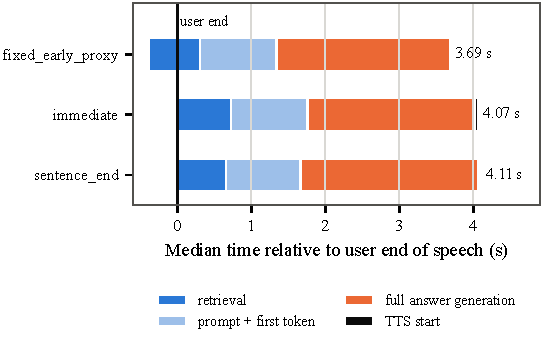
\includegraphics[width=\columnwidth]{fig_e2_latency_breakdown.pdf}
\caption{Median timeline of a v1 E2 turn relative to the user's end of speech,
per dispatch policy (250 runs each). Segment boundaries are medians of each
stage's timestamp, so segments are not additive. First audio starts only after
the full answer has been generated.}
\label{fig:latency}
\end{figure}

\subsection{Coupling Value (E3)}\label{sec:v1-e3}
% ---- P-VI.3 pre-registered verdict ----------------------------------------------
% PURPOSE: the pre-registered result, stated first and plainly.
% CLAIMS + EVIDENCE: 0 of 5 seeds show strict dominance of Ours over B9;
%   0 dominated operating points of 26 in every seed; reported as a tie, the
%   pre-registered second outcome [analysis/e3_dominance.json; PRE].
% NUMBERS: 0 of 5; 0 of 26.
\todo{P-VI.3: pre-registered E3 verdict (tie).}

% ---- P-VI.4 frontiers and baselines (Figs. 2a/2b, Table) -------------------------
% PURPOSE: show the real frontiers (R1 figures; R1.9 B4/B6/B8 results; replace
%   "dramatically outperform" with numbers).
% CLAIMS + EVIDENCE (Table~\ref{tab:v1e3}, Fig.~\ref{fig:frontiers}):
%   (a) Ours and B9 coincide at low prices: at lambda_l = 0.022 both have
%       accuracy 0.616 [0.488, 0.744], 0.82 retrievals per turn, p95 5.15 s
%       pooled; per seed, accuracy 0.58 to 0.66 and p95 4.60 to 5.51 s
%       [PN e3.pooled_operating_points, e3.per_seed]. (The figure "0.58,
%       0.82, 5.5 s" quoted in planning notes is seed 11 only.)
%   (b) Retrieval itself helps: B0 0.408 [0.284, 0.536]; best priced point
%       0.708; B8 0.708 [0.584, 0.824] at 0.68 retrievals/turn; B6 0.636 at
%       0.76; B4 is identical to B0 in every record because its threshold
%       (0.5) exceeds the largest value its signal takes (0.251), so it never
%       fires; it is reported as degenerate, not as a baseline result
%       [PN e3.b4_identical_to_b0; simulator/e3_scenario_signals.json].
%   (c) B4, B6 and B8 thresholds were fixed defaults, not swept on a dev
%       split, contrary to the pre-registered tuning protocol; say so
%       [configs/config.yaml controller.e3 comments; b8_independent.py
%       "still un-swept"]. B8's apparent edge over the priced controllers is
%       within the intervals.
%   (d) "Retrievals per dialogue" in the submission is retrievals per TURN
%       (single-turn scenarios) (R1 minor) [analysis/e3_frontier.py compute =
%       mean retrievals].
% NUMBERS: as in (a)--(b) and Table~\ref{tab:v1e3}.
\todo{P-VI.4: the frontiers of Fig.~\ref{fig:frontiers} and the baseline
points of Table~\ref{tab:v1e3}, including the degenerate B4 and the untuned
thresholds.}

% Table -- v1 E3 operating points (REAL sweep; pooled over 5 seeds x 50
% scenarios = 250 turns; 95% CI = scenario-cluster bootstrap, 2,000 draws).
% Every number: analysis/paper_v1_numbers.json -> e3.pooled_operating_points
%   (b0, b4, b6, b8; ours[i], b9[i] with i = grid index), generated by
%   `python -m analysis.paper_figures_v1` from simulator/e3_sweep_results/.
% Per-seed ranges (e3.unpriced_ranges): B0 acc 0.40-0.42; B6 0.60-0.68 at
%   0.76 retrievals/turn; B8 0.68-0.74 at 0.68.
% R1.9: B4/B6/B8 results; B4 identical to B0 in every record
%   (e3.b4_identical_to_b0 = true; its threshold 0.5 exceeds the maximum of
%   its signal, 0.251, on all 50 scenarios: simulator/e3_scenario_signals.json).
\begin{table}[t]
\caption{v1 E3 Operating Points (Real Sweep, 50 Scenarios $\times$ 5 Seeds;
95\% Scenario-Cluster Bootstrap Intervals)}
\label{tab:v1e3}
\centering
\footnotesize
\setlength{\tabcolsep}{2.5pt}
\resizebox{\columnwidth}{!}{%
\begin{tabular}{@{}l c c c c@{}}
\toprule
Controller & $\lamL$ & Accuracy & p95 TTFA (s) & Retr./turn\\
\midrule
B0 never & -- & 0.408 [0.284, 0.536] & 2.67 [2.36, 3.08] & 0.00\\
B4 (= B0) & -- & 0.408 [0.284, 0.536] & 2.67 [2.36, 3.08] & 0.00\\
B6 DRAGIN-style & -- & 0.636 [0.512, 0.768] & 5.78 [5.18, 6.06] & 0.76\\
B8 indep.-best & -- & 0.708 [0.584, 0.824] & 5.15 [4.57, 5.92] & 0.68\\
\midrule
Ours = B9 & 0.022 & 0.616 [0.488, 0.744] & 5.15 [4.60, 5.92] & 0.82\\
Ours & 0.349 & 0.676 [0.552, 0.796] & 5.15 [4.57, 5.92] & 0.72\\
B9 & 0.349 & 0.696 [0.572, 0.816] & 5.15 [4.57, 5.92] & 0.70\\
Ours & 1.240 & 0.708 [0.588, 0.820] & 5.15 [4.55, 5.92] & 0.60\\
B9 & 1.240 & 0.620 [0.480, 0.744] & 4.53 [3.53, 5.05] & 0.32\\
Ours & 1.713 & 0.620 [0.480, 0.744] & 4.53 [3.53, 5.05] & 0.32\\
B9 & 1.713 & 0.408 [0.284, 0.536] & 2.62 [2.34, 3.06] & 0.00\\
\bottomrule
\end{tabular}%
}
\end{table}


\begin{figure*}[t]
\centering
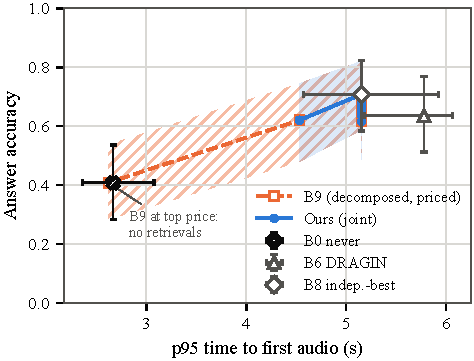
\includegraphics[width=0.49\textwidth]{fig_e3_acc_vs_p95.pdf}\hfill
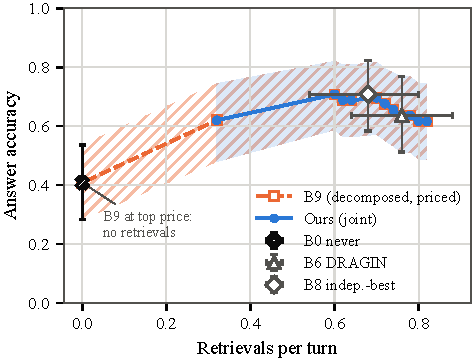
\includegraphics[width=0.49\textwidth]{fig_e3_acc_vs_compute.pdf}\\[-1mm]
\makebox[0.49\textwidth]{\footnotesize (a)}\hfill\makebox[0.49\textwidth]{\footnotesize (b)}
\caption{v1 E3 frontiers on the real sweep: answer accuracy against (a) p95
time to first audio and (b) retrievals per turn, for the joint controller
(Ours) and the decomposed controller (B9) over 26 latency prices, and for the
unpriced baselines B0, B6 and B8. Points pool 5 seeds $\times$ 50 scenarios;
shaded (Ours) and hatched (B9) bands and error bars are 95\% scenario-cluster
bootstrap intervals. B4 coincides with B0 and is not drawn. Per-seed panels
are in the supplementary material.}
\label{fig:frontiers}
\end{figure*}
% Supplementary: figures/fig_e3_per_seed.pdf (one panel per seed, R1
% figures: "or per-seed panels"). \PEND{supplementary material allowed?}

% ---- P-VI.5 why the frontiers coincide (Props. 1--2 on the data) ------------------
% PURPOSE: answer R1.1 with the data. IMPORTANT (coordinator correction,
%   2026-10-15): Ours(lambda_i) = B9(lambda_{i-1}) on the grid holds BY
%   CONSTRUCTION -- simulator/e3_grid.py tiles divergence bands edge to edge,
%   so the grid is geometric about lambda_deg = 0.021277 with ratio
%   L/(L - o*) = 1.3884 -- and is an implementation check, NOT evidence.
% CLAIMS + EVIDENCE (the evidence):
%   (a) The exact price map of Prop. 1 reproduces 10,000/10,000 decisions on
%       200 off-grid prices; the approximate map lambda(L - o*)/L gets
%       9,938/10,000 and fails at 46 prices, because of the waste term
%       [V1T prop1_dense].
%   (b) B9+ reproduces Ours on all 11,300 decisions checked (1,300 grid +
%       10,000 dense) [V1T b9plus].
%   (c) The divergence band is non-empty at 11 of 26 prices and contains 41
%       of 1,300 scenario-price decisions (3.15%); at every price the
%       scenarios on which Ours and B9 disagree are exactly the in-band
%       scenarios (Fig.~\ref{fig:band}) [V1T band_summary].
%   (d) On the grid, Ours(lambda_i) and B9(lambda_{i-1}) agree on
%       1,250/1,250 retrieve decisions and 941/941 timings; accuracy and
%       compute agree at 125/125 seed-price points, p95 TTFA at 123/125
%       (max difference 84 ms, a logging artefact: skipped turns are read
%       from per-timing skip cells) (Fig.~\ref{fig:shift})
%       [V1T prop1_on_grid] -- present as a check that the implementation
%       matches the theory.
%   (e) B9 at the top price (1.713) retrieves on 0 of 50 turns: its cut
%       (1.201) exceeds every belief, so it is disabled rather than beaten
%       [V1T band_per_price[25]; PN e3.b9_top_price].
% NUMBERS: 10,000/10,000; 9,938; 46; 200; 11,300; 11 of 26; 41 of 1,300;
%   3.15%; 1,250; 941; 125/125; 123/125; 84 ms; 0.021277; 1.3884; 0 of 50;
%   1.201.
\todo{P-VI.5: the equivalence on the v1 data: exact price map, \Bplus,
band occupancy (Fig.~\ref{fig:band}), and the grid shift of
Fig.~\ref{fig:shift} as an implementation check that holds by construction.}

\begin{figure}[t]
\centering
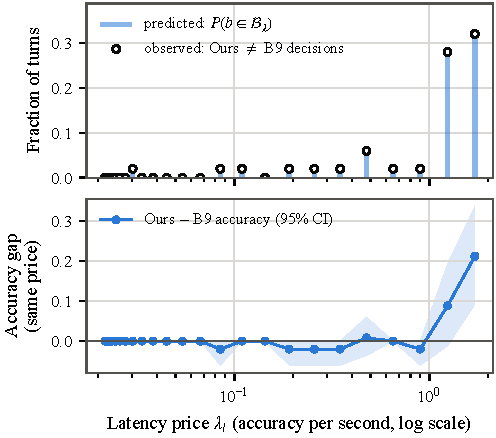
\includegraphics[width=\columnwidth]{fig_e3_band_occupancy.pdf}
\caption{Divergence band of Eq.~(\ref{eq:band}) on the v1 sweep. Top: fraction
of the 50 scenarios whose belief lies in the band at each latency price (bars)
and fraction on which Ours and B9 decide differently (circles); they coincide
at all 26 prices. Bottom: accuracy of Ours minus B9 at the same price, with a
95\% scenario-cluster bootstrap band.}
\label{fig:band}
\end{figure}

\begin{figure}[t]
\centering
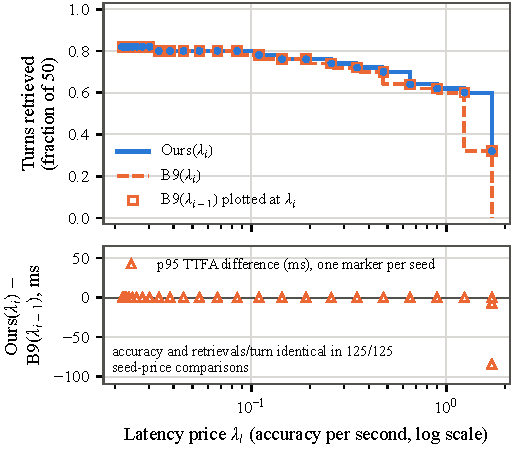
\includegraphics[width=\columnwidth]{fig_e3_price_shift.pdf}
\caption{Price shift on the v1 grid. Top: fraction of turns retrieved by Ours
at $\lambda_i$ and by B9 at $\lambda_i$ and at $\lambda_{i-1}$. Bottom:
Ours$(\lambda_i)$ minus B9$(\lambda_{i-1})$ in p95 TTFA for each seed. The
grid was built so that this shift holds exactly (consecutive bands tile edge
to edge), so the figure checks the implementation; it is not independent
evidence for Proposition~\ref{prop:eq}.}
\label{fig:shift}
\end{figure}

% ---- P-VI.6 the size and sign of the gap; the cost model -------------------------
% PURPOSE: Prop. 2 against the data; why the controller's own model is wrong
%   (corrected objective; measured latency). Keeps the null central (R2).
% CLAIMS + EVIDENCE:
%   (a) Accuracy gap Ours - B9 at the same price is -0.020 at five
%       single-scenario band prices (a not-needed scenario with a high
%       belief enters the band) and +0.212 [0.092, 0.340] at the top price,
%       the only price whose interval excludes zero [V1T prop2, prop2_summary].
%   (b) The v1 controller model predicts a non-negative gap everywhere; the
%       corrected objective (Eq. obj with measured g^+/g^-) predicts the
%       observed accuracy gaps with Pearson 0.975 over the 11 band prices
%       [V1T prop2_summary.corr_pred_corrected_vs_obs_acc].
%   (c) Measured TTFA cost of retrieving (paired retrieve minus skip) is
%       1.57 s at sentence_end and 1.20 to 1.30 s at the early timings
%       (1.20/1.27 s fixed_early_proxy and 1.25/1.30 s immediate, against the
%       sentence_end skip cell / the same-timing skip cell),
%       against the controller's 0.672 s and 0.484 s: the v1 cost model
%       understated it by more than a factor of two [V1T measured_latency].
%   (d) With the corrected objective and the measured cost, predicted and
%       observed realised-utility gaps agree in sign at 10 of 11 band prices
%       (Pearson 0.952); the v1 model gets the sign right at 1 of 11. Priced
%       at the measured latency, Ours's accuracy win at the top price is a
%       utility LOSS of -0.479 [-0.819, -0.175] [V1T prop2[25],
%       prop2_summary.utility_pred_measured_vs_obs].
% NUMBERS: -0.020 (x5), +0.212 [0.092, 0.340], 0.975, 1.57, 1.20-1.27,
%   1.30, 0.672, 0.484, 10 of 11, 0.952, 1 of 11, -0.479 [-0.819, -0.175].
\todo{P-VI.6: the signed gap, the corrected objective's prediction, and the
measured cost of retrieval that the v1 model understated.}
